\subsection{Decorator}
\subsubsection{Định nghĩa}
Decorator là một mẫu thiết kế cấu trúc (structural design pattern) cho phép bổ sung các tính năng mới vào một đối tượng mà không làm thay đổi cấu trúc của lớp gốc. Nó cho phép mở rộng chức năng của một đối tượng bằng cách đóng gói nó vào trong một lớp decorator mới và gắn kết chúng với nhau theo cấu trúc lồng nhau.
\subsubsection{Cách sử dụng}
Chúng ta sẽ sử dụng Decorator khi:
\begin{itemize}
    \item Khi muốn thêm tính năng mới cho các đối tượng mà không ảnh hưởng đến các đối tượng này.
    \item Khi bạn muốn mở rộng chức năng của một đối tượng mà không ảnh hưởng đến các đối tượng khác cùng loại.
    \item Khi không thể mở rộng một đối tượng bằng cách thừa kế (inheritance). Chẳng hạn, một class sử dụng từ khóa final, muốn mở rộng class này chỉ còn cách duy nhất là sử dụng decorator.
\end{itemize}
\subsubsection{Cấu trúc}
Các thành phần chính:
\begin{itemize}
    \item Một interface quy định mẫu dùng chung cho các sản phẩm
    \item Các sản phẩm kế thừa interface.
    \item Một abstract class có tham chiếu đến đối tượng sản phẩm và phương thức của interface quy định mẫu sản phẩm.
    \item Các Decorator con được kế thừa.
\end{itemize}
\begin{center}
    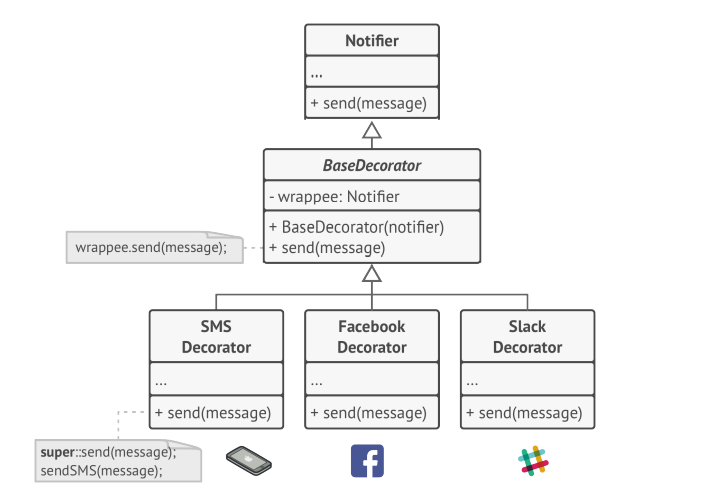
\includegraphics[scale=0.6]{image/structural/decorator.png}
\end{center}
\begin{itemize}
    \item Kiển trúc này thực chất là sau mỗi lần kế thừa, ta thêm vào các thuộc tính hoặc làm mới hàm mà vẫn giữ các giá trị của hảm cũ thì đó gọi là decorator.
\end{itemize}
\subsubsection{Ưu điểm và Nhược điểm}
Ta có các ưu và nhược điểm dễ thấy sau:\\\\
Ưu điểm:
\begin{itemize}
    \item Cho phép mở rộng chức năng của một đối tượng mà không làm thay đổi cấu trúc của lớp gốc.
    \item Có thể kết hợp nhiều decorator để tạo ra các kết hợp chức năng phức tạp.
    \item Bạn có thể mở rộng hành vi của đối tượng mà không cần tạo lớp con mới.
    \item Cung cấp tính linh hoạt và tùy chỉnh cao khi thêm hoặc xóa chức năng mà không ảnh hưởng đến các đối tượng khác.
\end{itemize}
Nhược điểm:
\begin{itemize}
    \item Dễ dẫn đến việc tạo ra quá nhiều lớp decorator nhỏ, dẫn đến sự phức tạp và khó khăn trong việc quản lý.
\end{itemize}
\subsubsection{Code Example}
\begin{itemize}
    \item Có 1 loại nước uống là Coffee.
    \item Có 2 loại trang trí đi kèm là Milk và Sugar.
\end{itemize}
\begin{lstlisting}
#include <iostream>
#include <string>

// Component interface
class Beverage {
public:
    virtual std::string getDescription() const = 0;
    virtual double getCost() const = 0;
};

// Concrete component
class Coffee : public Beverage {
public:
    std::string getDescription() const override {
        return "Coffee";
    }

    double getCost() const override {
        return 2.0;
    }
};

// Decorator
class BeverageDecorator : public Beverage {
protected:
    Beverage* beverage;

public:
    BeverageDecorator(Beverage* beverage) : beverage(beverage) {}

    std::string getDescription() const override {
        return beverage->getDescription();
    }

    double getCost() const override {
        return beverage->getCost();
    }
};

// Concrete decorators
class MilkDecorator : public BeverageDecorator {
public:
    MilkDecorator(Beverage* beverage) : BeverageDecorator(beverage) {}

    std::string getDescription() const override {
        return beverage->getDescription() + ", Milk";
    }

    double getCost() const override {
        return beverage->getCost() + 0.5;
    }
};

class SugarDecorator : public BeverageDecorator {
public:
    SugarDecorator(Beverage* beverage) : BeverageDecorator(beverage) {}

    std::string getDescription() const override {
        return beverage->getDescription() + ", Sugar";
    }

    double getCost() const override {
        return beverage->getCost() + 0.25;
    }
};

int main() {
    Beverage* coffee = new Coffee();
    std::cout << "Order: " << coffee->getDescription() << std::endl;
    std::cout << "Cost: $" << coffee->getCost() << std::endl;

    Beverage* coffeeWithMilk = new MilkDecorator(coffee);
    std::cout << "Order: " << coffeeWithMilk->getDescription() << std::endl;
    std::cout << "Cost: $" << coffeeWithMilk->getCost() << std::endl;

    Beverage* coffeeWithMilkAndSugar = new SugarDecorator(coffeeWithMilk);
    std::cout << "Order: " << coffeeWithMilkAndSugar->getDescription() << std::endl;
    std::cout << "Cost: $" << coffeeWithMilkAndSugar->getCost() << std::endl;

    delete coffee;
    delete coffeeWithMilk;
    delete coffeeWithMilkAndSugar;

    return 0;
}

\end{lstlisting}
Ở hàm main, ta gọi 1 tách cà phê và xem thông tin của nó. Sau đó, tiếp tục gọi 1 tách cà phê thêm đường. Cuối cùng là 1 tách cà phê thêm đường và sửa.\\
\newline
\textbf{Kết quả:}
\begin{lstlisting}
Order: Coffee
Cost: $2
Order: Coffee, Milk
Cost: $2.5
Order: Coffee, Milk, Sugar
Cost: $2.75

\end{lstlisting}
\subsubsection{Các Pattern liên quan}
\begin{itemize}
    \item Adapter: Decorator thực chất không hề thay đối nội dung của đối tượng mà mở rộng hay thay đối trách nhiệm của đối tượng đó.
    \item Composite: khá giống nhau về mặt cấu trúc tuy nhiên decorator thêm các hành vi cụ thể hoặc cải tiến nó còn composite thì không.
    \item Strategy cho phép bạn thay đối nội dung của đối tượng trong khi decorator vẫn giữ nguyên.
\end{itemize}